% Author: Ladislav Vašina <xvasin11@stud.fit.vutbr.cz>

\documentclass[12pt, a4paper]{article}
\usepackage{indentfirst}
\usepackage[czech]{babel}
\usepackage[utf8]{inputenc}
\usepackage[left=2cm, top=3cm, text={17cm, 24cm}]{geometry}
\usepackage{times}
\usepackage{verbatim}
\usepackage{enumitem}
\setenumerate[1]{label=\arabic*)}
\usepackage{graphicx}
\usepackage[unicode]{hyperref}
\usepackage{pdfpages}
\usepackage{caption}
\usepackage{tabularx, booktabs} 
\usepackage{amsmath,bm}

\hypersetup{
	colorlinks = true,
	hypertexnames = false,
	citecolor = red
}

\begin{document}
	% Titulní stránka 
	\begin{titlepage}
		\begin{center}
			
\includegraphics[width=0.77\linewidth]{images/fit_logo.png} \\

			\vspace{\stretch{0.382}}

			\Huge{\textbf{ESP32: Měření srdečního tepu}} \\ 
            \LARGE{Mikroprocesorové a vestavěné systémy}
			\vspace{\stretch{0.618}}
		\end{center}

		\begin{minipage}{0.4 \textwidth}
			{\Large \today}
		\end{minipage}
		\hfill
		\begin{minipage}[r]{0.6 \textwidth}
			\Large
			\begin{tabular}{l l l}
				Ladislav Vašina & (xvasin11)
			\end{tabular}
		\end{minipage}
	\end{titlepage}
	
	% Obsah
	\setcounter{page}{1}
	\addtocontents{toc}{\protect\thispagestyle{empty}}
	\tableofcontents
	\clearpage
	
    \section{Úvod}
    Tento dokument popisuje řešení projektu do kurzu Mikroprocesorové a vestavěné systémy na Fakultě informačních technologií. 
    
    Cílem projektu bylo implementovat měřič srdečního tepu s využitím vývojové platformy na bázi SoC ESP32. Tep je snímán pomocí snímače MAX30102 \cite{MAX30102} a aktuální hodnoty tepu jsou zobrazovány na OLED displej ssd1306 \cite{ssd1306}. Navíc bylo implementováno i rozšíření, a to takové, že se modul ESP32 využije jako AP, jenž vytvoří vlastní web server, na kterém jsou asynchronně zobrazovány naměřené hodnoty.

    Při implementaci bylo využito editoru Visual Studio Code a jeho rozšíření Platformio \cite{platformio}.
    Projekt byl vytvořen za použití frameworku Arduino (zvolen z důvodu vyšší kvality knihoven pro naše komponenty) a těchto 3 knihoven:
    \begin{itemize}
        \item \textbf{Adafruit\_SSD1306} \cite{adafruitSsd1306} (Knihovna pro práci s displejem ssd1306)
        \item \textbf{Adafruit-GFX-Library} \cite{adafruitGFX} (Knihovna pro práci s displejem ssd1306)
        \item \textbf{SparkFun\_MAX3010x\_Sensor\_Library} \cite{sparkfun} (knihovna pro práci se senzorem MAX30102)
    \end{itemize}
    \subsection{Zapojení komponent}
    Displej ssd1306 je zapojen pomocí rozhraní SPI a senzor tepu je zapojen pomocí rozhraní I2C. Obě tyto komponenty jsou napájeny pomocí napětí 3.3 V
    \begin{figure}[ht]
		\centering
		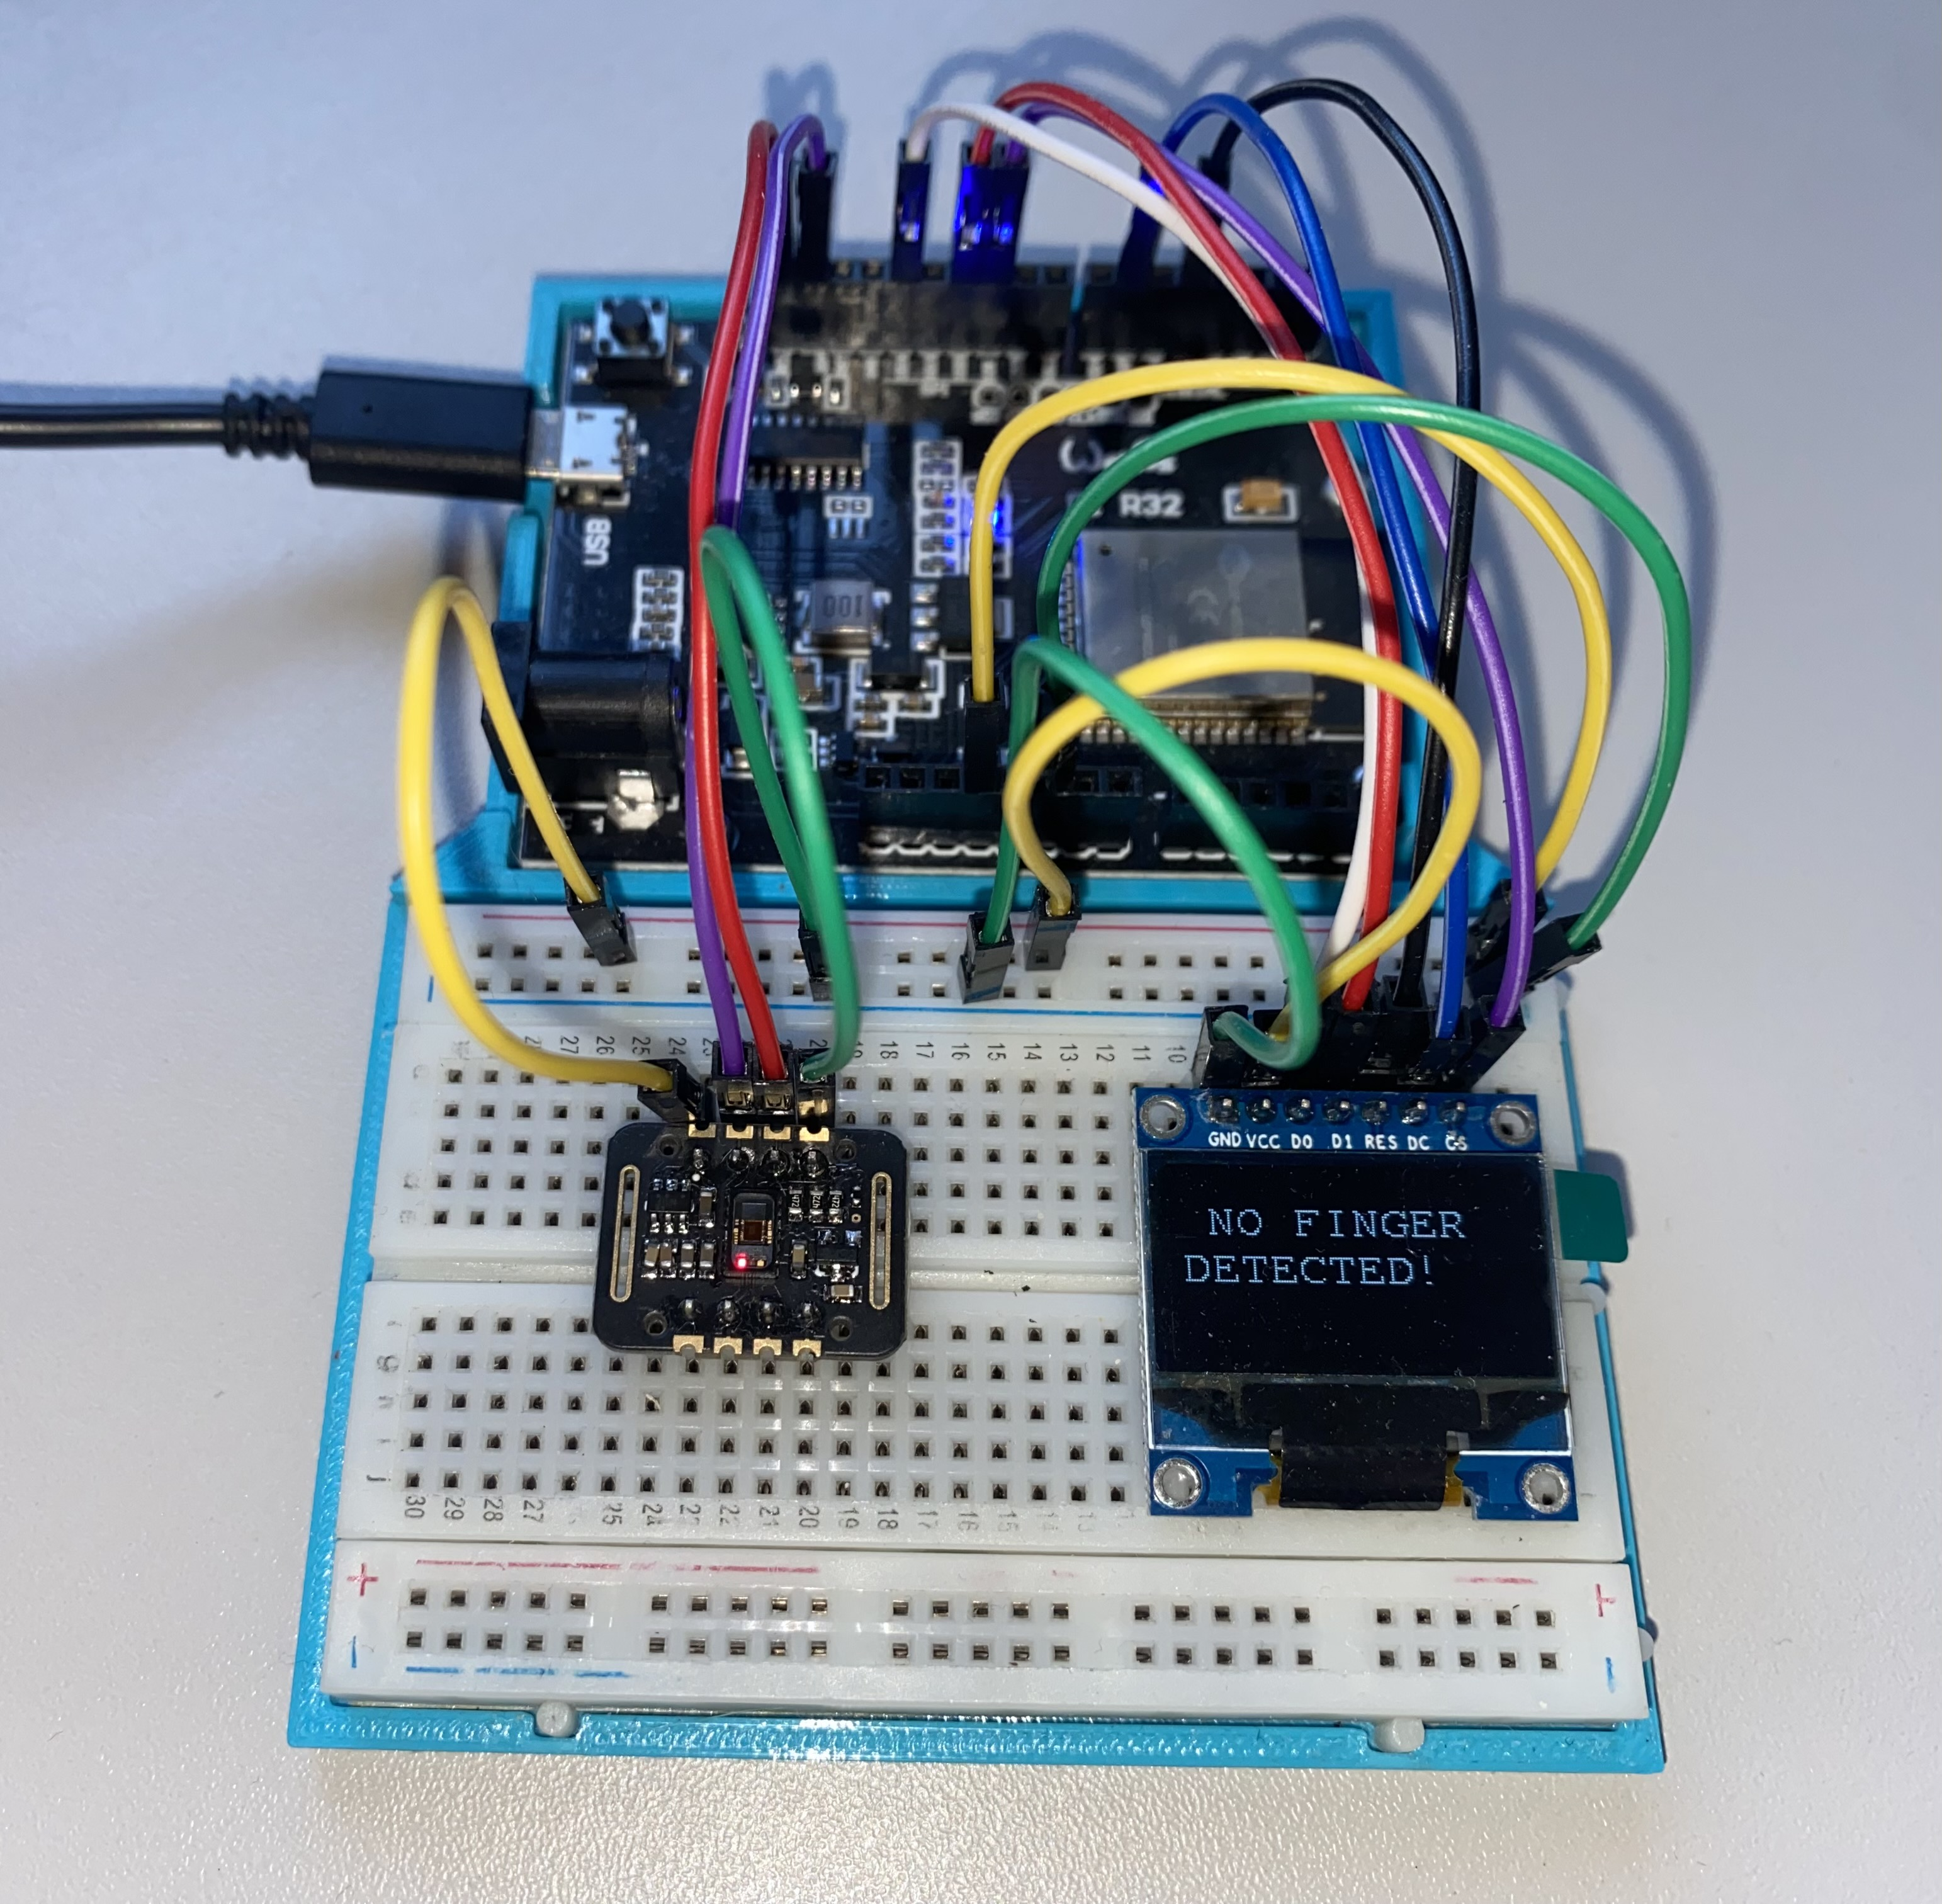
\includegraphics[width=0.6\linewidth]{images/zapojeni.jpeg}\newline
	    \caption{Detail zapojení desky}
	\end{figure}
    \subsection{Vlastní způsob spuštění projektu}
    Je nutné mít nainstalovaný editor Visual Studio Code s nainstalovaným rozšířením Platformio. Následně se klikne na ikonu rozšíření Platformio v levém panelu VSC, kde zvolíme možnost\newline \texttt{Quick Access/PIO Home/Open --> New Project}. Dále se nám zobrazí dialogové okno pro vytvoření projektu. Zadáme jméno nového projektu, ve výběru \uv{Board} vybereme \texttt{Espressif ESP32 Dev Module} a možnost \uv{Framework} ponecháme Arduino a klikneme na tlačítko \texttt{finish}. Následně se nám zobrazí struktura projektu a soubor \texttt{platformio.ini}. Do tohoto souboru nakonec dopíšeme řetězec \texttt{monitor\_speed = 115200}.
    
    Do složky \texttt{src} v našem nově vytvořeném projektu vložíme zdrojové soubory tohoto projektu \texttt{main.cpp} a \texttt{index.h}.
    
    Dále je nutné si doinstalovat do projektu potřebné knihovny. To provedeme tak, že se klikne na ikonu rozšíření Platformio v levém panelu VSC, kde zvolíme možnost\newline \texttt{Quick Access/PIO Home/Libraries}. Mělo by se nám zobrazit vyhledávací pole, kde postupně vyhledáme tyto 3 knihovny: 
    Adafruit SSD1306, Adafruit GFX Library,\newline SparkFun MAX3010x Pulse and Proximity Sensor Library. Každou z těchto knihoven je potřeba po vyhledání přidat do nově vytvořeného projektu. Následně již stačí připojit naší ESP32 desku se správně zapojenými komponentami a zvolit možnost \texttt{Upload and Monitor} v levém panelu editoru VSC.
    \section{Popis řešení}
    Samotné řešení projektu se nachází v souborech \texttt{main.cpp} a \texttt{index.h}.

    
    Soubor \texttt{main.cpp} obsahuje všechny funkce, které řídí měření tepu, zobrazování dat na displej či spuštění webového serveru.

    Soubor \texttt{index.h} obsahuje strukturu zobrazované webové stránky na web serveru a skript využívající asynchronní komunikace pro zobrazování aktualizovaných dat na webu.
    \subsection{Funkce \texttt{setup}}
    Na počátku této funkce se vytváří proměnné potřebné k inicializaci snímače tepu. Snímač tepu je inicializován např. s hodnotou intenzity svitu LED diody, či módem svitu (jen červená led/ infračervená + červená led) apod. Vstupní proud diod je nastaven na cca 6,25 mA. Při vyšším proudu již nedokáže snímač kvalitně rozeznat změny ve snímaných hodnotách. Dále se inicializuje displej, na kterém budeme zobrazovat měřené hodnoty a pomocí knihovních funkcí nastavíme vlastní font, velikost, barvu, kódování zobrazovaného textu a místo pozici na displeji kam budeme chtít vykreslovat údaje.
    
    \subsection{Funkce \texttt{loop}}
    Tato funkce je hlavní smyčkou programu, ve které se nachází samotný výpočet uživatelova srdečního tepu. Výpočet funguje tak, že se pomocí knihovní funkce \texttt{checkForBeat} kontroluje, zda byl zachycen úder srdce. Pokud tomu tak je, vypočítá se čas $\bm{\Delta t}$ \textbf{[ms]} od posledního zachyceného úderu srdce. Počet úderů srdce za minutu je následně vypočítán tímto vztahem $\bm{BpM = \frac{60}{\Delta t / 1000}}$.\newline
    Dále se také ze zachycených hodnot \texttt{BpM} vypočítá průměrná hodnota uživatelova tepu. Ta se počítá tak, že máme vytvořené pole o velikosti 8, které postupně naplňujeme hodnotami \texttt{BpM}. Z těchto hodnot je následně vypočítána průměrná hodnota uživatelova tepu.
    Dále můžeme z přečtených hodnot snímače zjistit, zda se uživatel dotýká senzoru či nikoliv. Pokud tedy zjistíme, že je hodnota pod nějakou úroveň, tak voláme funkci \texttt{printDisplayNoFinger} \ref{subsection:printDisplayNoFinger}. V opačném případě začneme vypisovat hodnoty na displej voláním funkce \texttt{printDisplayInfo} \ref{subsection:printDisplayInfo}. Na konci funkce \texttt{loop} voláme knihovní funkci \texttt{handleClient}, která obslouží klienta, který se chce připojit k našemu web serveru.
    
    \subsection{Funkce \texttt{printDisplayInfo}}
    \label{subsection:printDisplayInfo}
    Funkce \texttt{printDisplayInfo} přijímá jako vstupní parametry počet tepů srdce za minutu a průměrný uživatelův tep. Tyto hodnoty se pomocí knihovních funkcí zobrazují na připojeném OLED displeji. Na počátku funkce se musí displej vymazat pomocí funkce \texttt{clearDisplay}.
    
    \subsection{Funkce \texttt{printDisplayNoFinger}}
    \label{subsection:printDisplayNoFinger}
    Tato funkce zobrazuje uživateli informaci, že není ke snímači přiložen prst. K zobrazení této informace se využívá funkcí z knihovny \texttt{Adafruit\_SSD1306} \cite{adafruitSsd1306}.
    
    \subsection{Funkce \texttt{webServerInit}}
    \label{subsection:webServerInit}
    V této funkci se nastavuje WiFi mód našeho zařízení. Tento mód nastavíme na AP tímto \newline příkazem: \texttt{WiFi.mode(WIFI\_AP)}. Dále je nastaveno jméno naší WiFi sítě, které je nastaveno na \texttt{XVASIN11-ESP32-AP}. WiFi nemá nastavené žádné heslo pro jednodušší přístup. Dále je zavolána funkce \texttt{handleRoot} \ref{subsection:handleRoot}, která na web načte HTML strukturu stránky ze souboru \texttt{index.h} s asynchronním skriptem, který aktualizuje informace na webu. Nakonec je zavolána funkce \texttt{handleWeb}, která zašle aktualizovaná data na web.
    
    \subsection{Funkce \texttt{handleRoot}}
    \label{subsection:handleRoot}
    Funkce načte ze souboru \texttt{index.h} HTML strukturu a tu zašle na server.
    \subsection{Funkce \texttt{handleWeb}}
    \label{subsection:handleWeb}
    Tato funkce zašle aktualizovaná data o uživatelově tepové frekvenci v text/plain formátu na web server.
    \newpage
    \subsection{ROZŠÍŘENÍ - Popis webového serveru}
    \label{subsection:pipisWebovehoServeru}
    Po připojení napájení do naší platformy na bázi SoC ESP32 se spustí, nejen měření tepu a displej zobrazující naměřené hodnoty, ale spustí se i webový server umožňují zobrazit si naměřené hodnoty na mobilním zařízení.
    
    Aby uživatel mohl číst tyto hodnoty musí se na svém mobilním zařízení připojit na WiFi síť s názvem \texttt{XVASIN11-ESP32-AP} (WiFi je bez hesla) a do prohlížeče zadat adresu \textbf{192.168.4.1}.
    Na této webové adrese bude uživateli zobrazen výstup měření jeho srdečního tepu.
    \begin{figure}[ht]
		\centering
		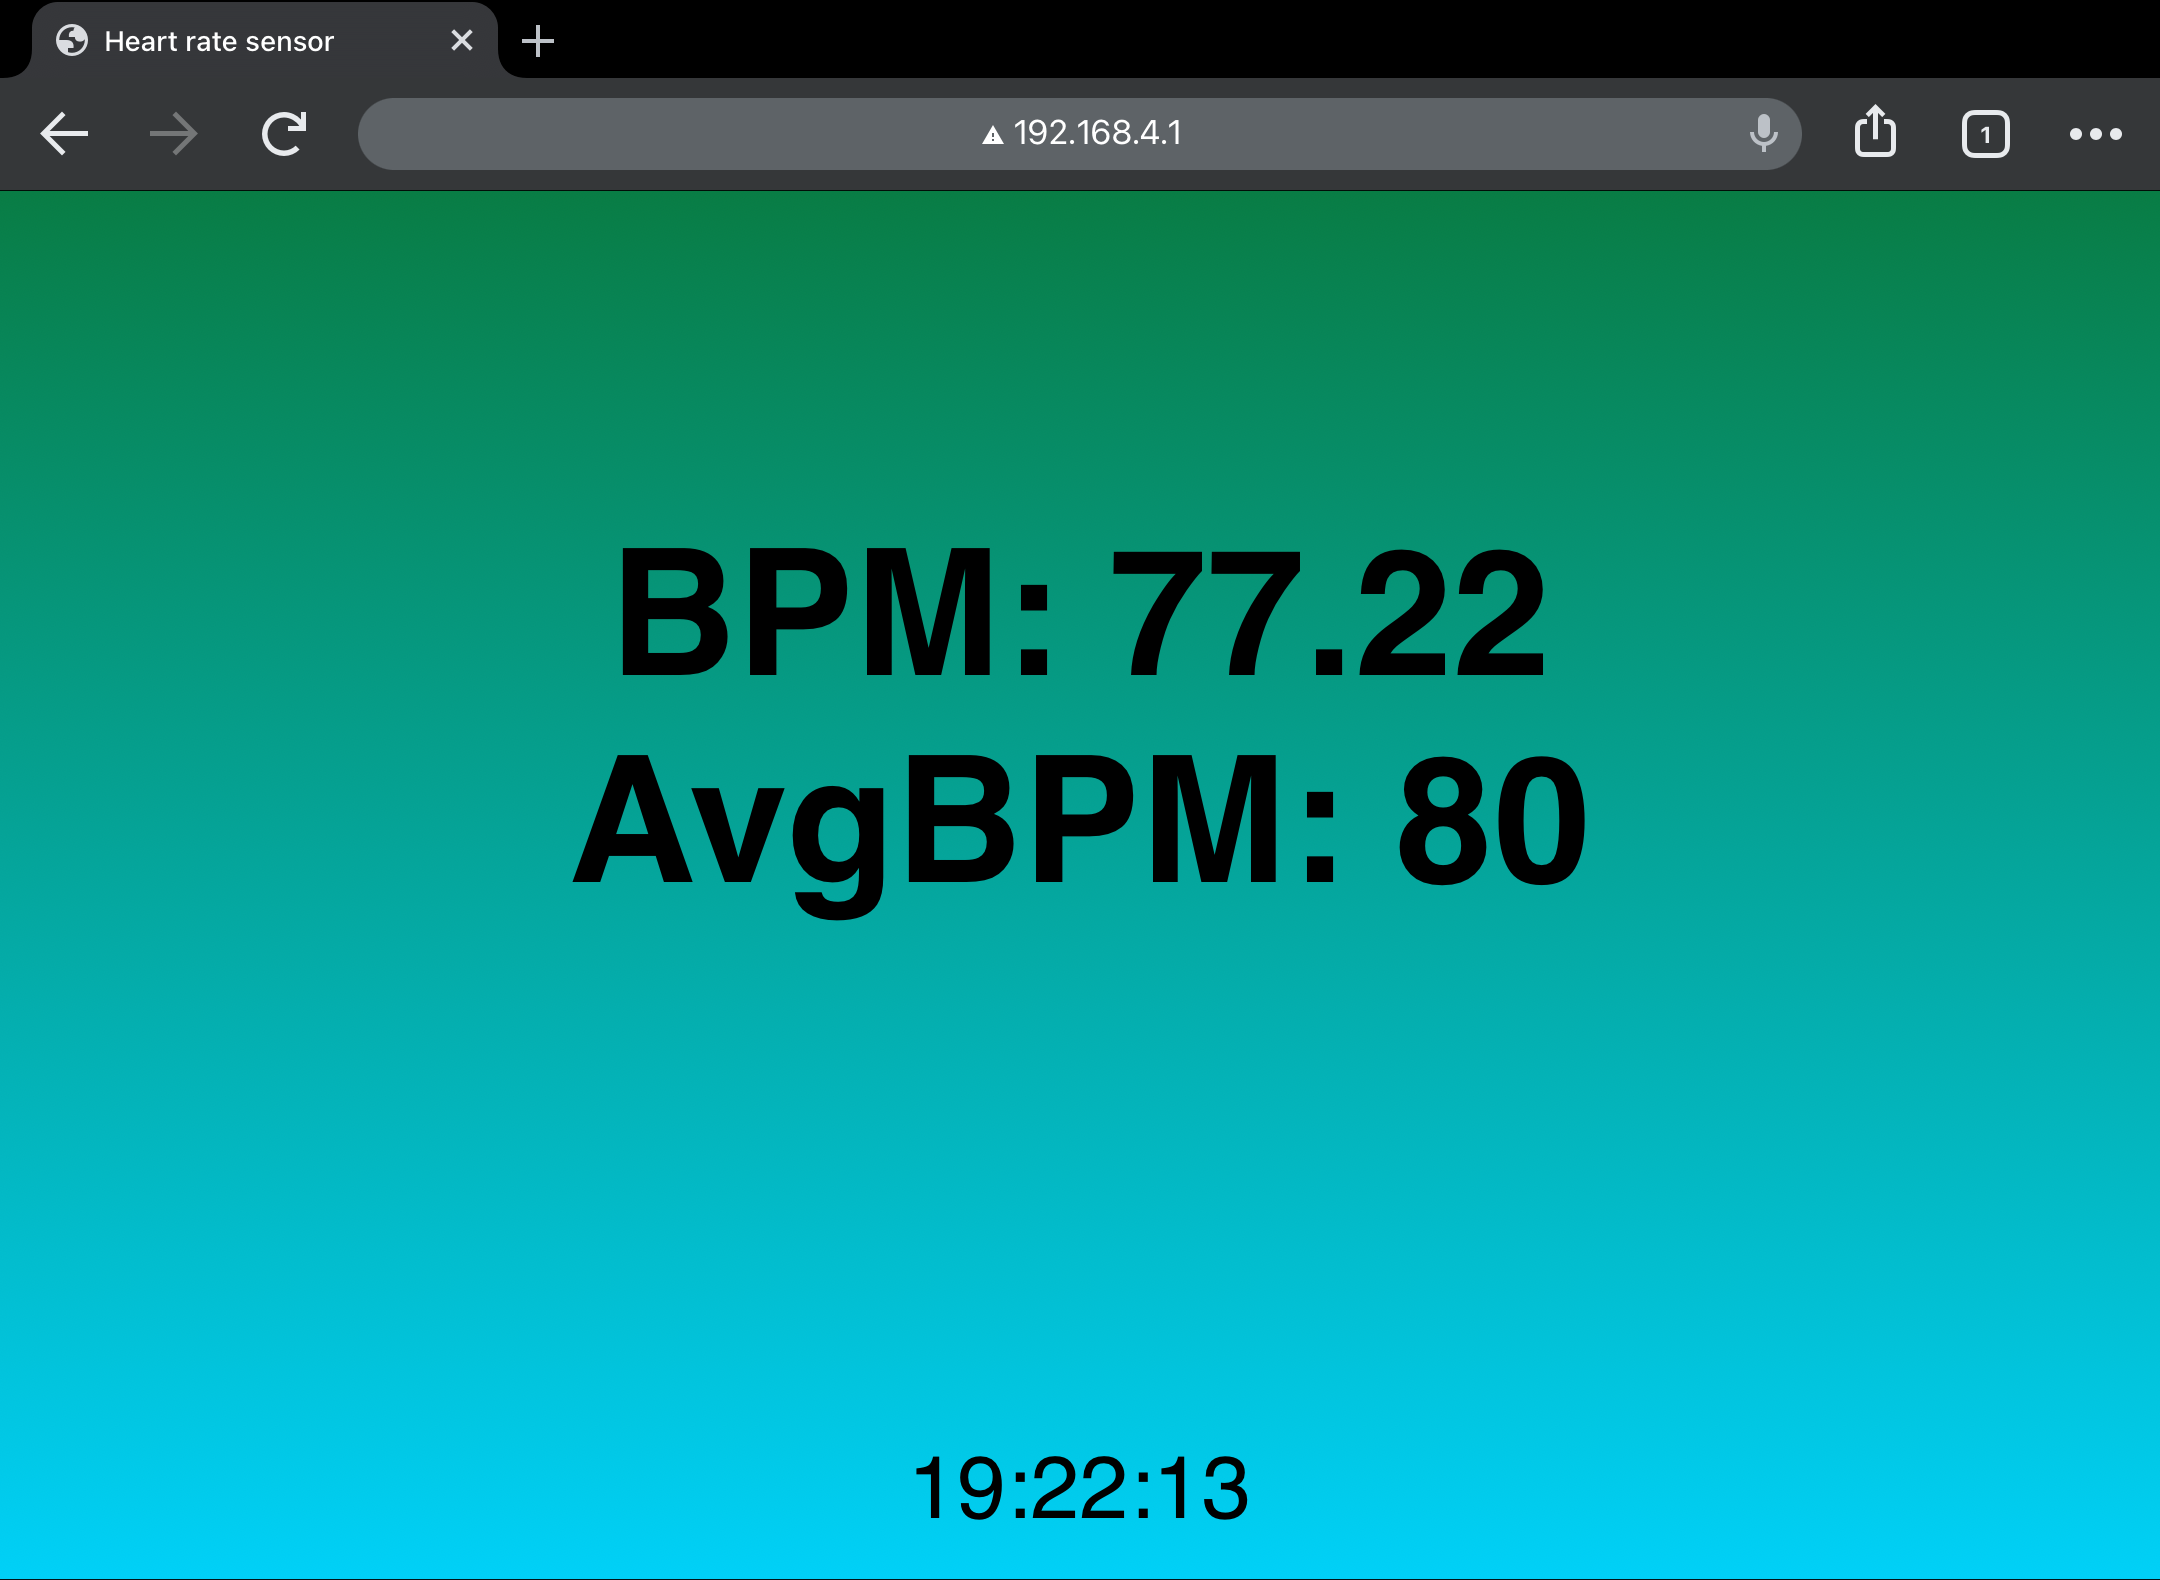
\includegraphics[width=0.9\linewidth]{images/webserver.png}\newline
	    \caption{Ukázka webového rozhraní AP}
	\end{figure}
    
    
    \section{Zhodnocení}
    Mnohými měření tepu jsem zjistil, že pro získání korektních a stabilních hodnot, je opravdu velmi důležité udržovat konstantní tlak na senzor tepu. Projekt mi jako takový nepřišel nějak moc složitý, proto jsem se rozhodl navíc implementovat zobrazení naměřených hodnot na vlastním web serveru viz \ref{subsection:pipisWebovehoServeru}.
    Ověření funkčnosti probíhalo simultánním měřením srdečního tepu na platformě ESP32 s využitím senzoru MAX30102 a na mobilním telefonu Samsung Galaxy S9, který má také senzor pro měření tepu. Po provedení tohoto paralelního měření byly získané hodnoty v celku podobné, z čehož usuzuji, že mé řešení měření tepu odpovídá realitě.

    \newpage
    \section{Video prezentující projekt}
    Níže jsou uvedené odkazy k videu prezentující funkční řešení projektu.
    \newline

    Odkaz na přehraní videa na YouTube: \href{https://youtube.com/shorts/GdGj5rN2Gnw?feature=share}{https://youtube.com/shorts/GdGj5rN2Gnw?feature=share}



    Odkaz na stažení daného videa z Google Drive:\newline\href{https://drive.google.com/file/d/1TznYSvp2Ogxsz00HByiR1h28raW7ji5f/view?usp=sharing}{https://drive.google.com/file/d/1TznYSvp2Ogxsz00HByiR1h28raW7ji5f/view?usp=sharing}
    \section{Autoevaluace}
    Celkové hodnocení je dáno tímto vztahem: $\Sigma = (K_1 + K_2 \cdot F/5) \cdot (E + F + Q + P + D)$
    
    Hodnoty jednotlivých složek mého projektu:
    \begin{itemize}
        \item Konstanty $\bm{K_1 = 0,25}$
        \item Konstanty $\bm{K_2 = 0,75}$
        \item Přístup $\bm{E = 1}$\newline
        Projekt jsem začal implementovat i dokončil s předstihem. Nad rámec zadání jsem implementoval webový server zobrazující naměřená data.
        \item Funkčnost $\bm{F = 5}$\newline
        Cílem projektu bylo implementovat systém pro měření srdečního tepu. Tuto informaci má implementace úspěšně měří a zobrazuje na připojený OLED displej i na webový server.
        \item Kvalita $\bm{Q = 3}$\newline
        Řešení projektu je pro uživatele velmi přívětivé. Uživateli stačí pouze připojit napájení a téměř okamžitě může začít měřit své hodnoty srdečního tepu. Dále je díky nezabezpečenému AP, velmi jednoduché se na AP připojit. Po přístupu na určenou adresu jsou uživateli okamžitě zobrazeny naměřené hodnoty. Zdrojové kódy jsou okomentovány a rozděleny do funkcí, což zajišťuje jejich přehlednost a čitelnost. Implementace projektu je dekomponována na menší problémy, které jsou řešeny v jednotlivých funkcích (zobrazování dat na displeji/webu apod.).
        \item Prezentace $\bm{P = 1}$\newline
        Video prezentující řešení plně zobrazuje funkčnost podle zadání i implementované rozšíření o webový server zobrazující měřené hodnoty.
        \item Dokumentace $\bm{D = 4}$\newline
        Dokumentace splňuje všechny požadované komponenty jako jsou úvod do problému, popis implementace a zhodnocení.
    \end{itemize}

    Po dosazení hodnot do výše uvedeného vzorce nám vyjde celkový počet bodů:\newline
    \begin{center}
        $\Sigma = (0,25 + 0,75 \cdot 5/5) \cdot (1 + 5 + 3 + 1 + 4) = \bm{14}$ \textbf{bodů}
    \end{center}
	\clearpage
	\bibliographystyle{czechiso}
	\renewcommand{\refname}{Použitá literatura}
	\bibliography{main}

\end{document}